\chapter{Inductive Synthesis of State Machines from Scenarios\label{chapter:inductive-synthesis}}

This chapter presents inductive techniques for synthesizing state machines from scenarios. Section~\ref{section:inductive-problem-statement} states the problem statement precisly and discusses requirements on the synthesis approach. Section~\ref{section:inductive-background} provides background on grammar induction \cite{Gold:1978}, the inductive framework on which techniques of the chapter rely. Section~\ref{section:lts-induction-from-mscs} then describes an interactive inductive technique for learning Labeled Transition Systems (LTS) from collections of Message Sequence Charts (MSC). This technique is guided by an end-user, which is expected to classify additional MSC scenarios as positive and negative system behaviors. Fluent, goals and domain properties may be injected to enforce inter-model consistency while pruning the induction search space. Section \ref{section:inductive-from-hMSC} describes a similar, yet non-interactive technique, to synthesize LTSs from high-level MSCs. Section \ref{section:inductive-discussion} concludes this chapter with a discussion about inductive synthesis of state machines and possible future directions. 

\section{Synthesis objectives and chosen approach\label{section:inductive-overview}}

This section gives an overview of the synthesis approach. Section~\ref{subsection:inductive-synthesis-statement} states the problem statement in terms of the formal models of Chapter~\ref{chapter:framework}. Section~\ref{subsection:inductive-synthesis-requirements} completes this by stating additional requirements on the synthesis approach. Section~\ref{subsection:inductive-synthesis-approach} presents our grammar induction oriented approach.

%%%

\subsection{Problem statement\label{subsection:inductive-synthesis-statement}}

In its simplest form, the LTS synthesis problem can be stated as follows:

\begin{quotation}
\noindent \underline{Given}~~a consistent scenario collection showing typical examples and counterexamples of system behaviors

\vspace{-0.7cm}
\begin{align*}
Sc = (S^+,S^-)
\end{align*}

\vspace{-0.2cm}
\noindent \underline{Synthesize}~~the system as a composition of agent LTSs

\vspace{-0.7cm}
\begin{align*}
System = (Ag_1 \parallel \ldots \parallel Ag_n)
\end{align*}

\vspace{-0.2cm}
\noindent \underline{Such that}~~$Sc$ and $System$ are consistent.
\end{quotation}

\noindent For recall, the consistency condition means that (see Section~\ref{subsection:background-scenario-consistency}):

\begin{itemize}
\item \textbf{structural consistency} -- the state machine and scenario views are \emph{structurally} consistent, that is, they agree on the agent decomposition and their respective interface,
\item \textbf{consistent agent views} -- the timelines of any positive scenario $P \in S^+$ specify existing paths in the corresponding agent state machines. The same applies for the precondition of any negative scenario $N \in S^-$.
\item \textbf{consistent system view} -- the system correctly accepts positive scenarios and preconditions of negatives ones. It also correctly rejects negative scenarios. We recall below the precise conditions from Section~\ref{subsection:background-scenario-consistency}:
\begin{align*}
\mathcal{L}(System) &= \mathcal{L}^+(Sc)\\
\mathcal{L}(System) \cap \mathcal{L}^-(Sc) &= \emptyset
\end{align*}

\end{itemize}

%%%

\subsection{Synthesis requirements\label{subsection:inductive-synthesis-requirements}}

The characterization above provides a \emph{minimal requirement} on the synthesis approach. Additional requirements are important to consider as well. Their inclusion depends on assumptions on input scenario models, the presence and/or absence of other models, the availability of an end-user, and so on.

\noindent \textbf{Richness of the scenario language} -- the richness of the input scenario language is an important issue for end-user involvement and usability of a synthesis approach:

\begin{itemize}

\item End-user are most likely to be unable to provide rich scenario descriptions in the early phases of system design. This includes state assertions along scenario episodes or flowcharts on such episodes. The synthesis approach should therefore work when only a few scenarios are available. 

\item Both positive and negative scenarios should be taken into account. Negative scenarios are not uncommon among the examples provided by stakeholders. One reason is that they naturally illustrate violations of safety goals while being easier to specify than the latter.

\item Given the incremental nature of tool-supported system analysis, richer input scenarios are however very likely to be \emph{eventually} available. Higher-level scenario models should therefore be supported as input of the synthesis technique for advanced analysis phases.

\end{itemize}

\noindent \textbf{Behavior generalization} -- the synthesis approach must at least cover the behaviors described in the positive scenarios. In most cases, scenarios provide \emph{examples} of system behaviors and are inherently incomplete. Synthesized state machines should therefore cover more behaviors than those already described. 

An upper bound on behavior generalization is entailed by the consistency condition, that requires negative scenarios to be correctly rejected. This upper bound has to be refined when other models are available (see below).

\noindent \textbf{Multi-model consistency} -- A argument similar to the one for high-level scenario models applies for other models. Fluents, goals and domain properties, etc. should not be \emph{required} as input, but are better \emph{supported} when available. 

In presence of multiple models, strengthening the characterization above is required. All available models shall be required to be consistent in input. In that case, the synthesis technique shall be such that synthesized LTSs are consistent with all input models. Notably, the synthesized system should not violate known safety goals.

%%%

\subsection{A grammar induction approach\label{subsection:inductive-synthesis-approach}}

Figure~\ref{image:inductive-synthesis-overview} shows the three main steps of our synthesis approach. We will assume here that a scenario collection $Sc = (S^+, S^-)$ is taken as input of the synthesis process. Adaptations of the first two steps below are required to take high-level MSCs as input; they will be covered in Section~\ref{section:inductive-from-hMSC}.

\begin{figure}\centering
  \scalebox{0.60}{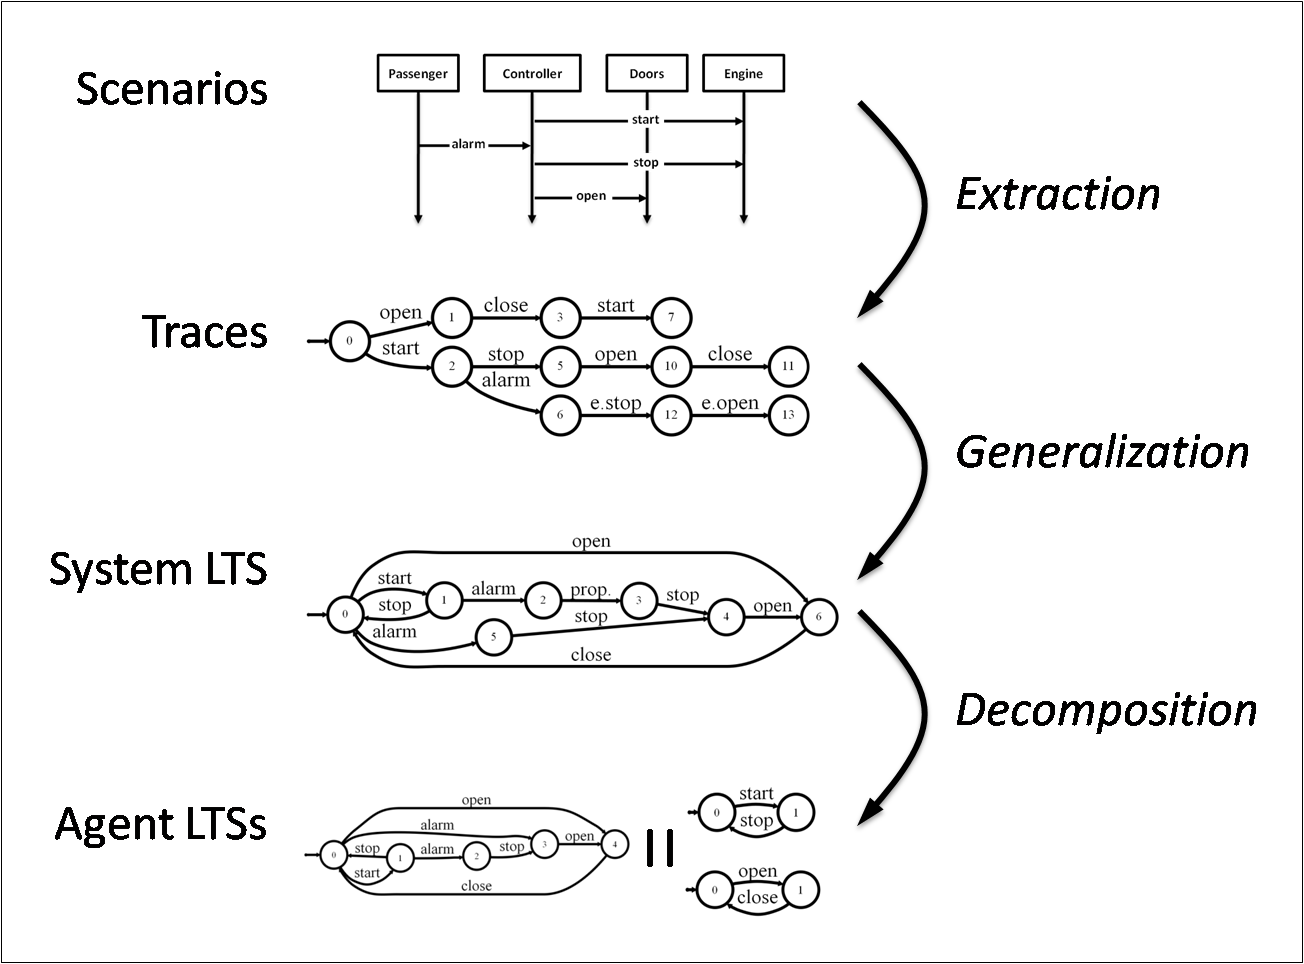
\includegraphics[trim=2mm 2mm 3mm 2mm, clip]{src/4-inductive/images/overview}}
  \caption{Overview of inductive LTS synthesis from MSCs.\label{image:inductive-synthesis-overview}}
\end{figure}

\noindent \textbf{Extraction} -- this step consists in extracting scenarios traces as a first automaton. The extraction relies on the trace semantics of scenarios given in Chapter~\ref{chapter:framework}. 

Traces are captured by a \emph{prefix tree acceptor} (PTA), the largest deterministic automaton that accepts exactly the positive behaviors. At this step, the \emph{consistent system view} condition already holds, but no generalization occurs yet:
\begin{align*}
\mathcal{L}(PTA) &= \mathcal{L}^+(Sc)\\
\mathcal{L}(PTA) \cap \mathcal{L}^-(Sc) &= \emptyset
\end{align*}

\noindent \textbf{Generalization} -- grammar induction is used at this step so as to fullfil the behavior generalization requirement. The Regular Positive and Negative Inference (RPNI) algorithm is used as a building block \cite{Oncina:1992} for synthesizing a system LTS from the PTA.

Starting from the PTA, this algorithm incrementally refines the current automaton by merging well chosen state pairs. The generalization is performed under the control of negative scenarios. The \emph{consistent system view} remains an invariant for any current solution $A$:
\begin{align*}
\mathcal{L}(A) &\subseteq \mathcal{L}^+(Sc)\\
\mathcal{L}(A) \cap \mathcal{L}^-(Sc) &= \emptyset
\end{align*}

This inductive approach is enhanced in two ways so as to fulfill additional requirements:

\begin{itemize}

\item An interactive feature supports the elicitation of additional, ``interesting'' scenarios that are not originally provided by the end-user. The latter is expected to classify generated scenarios as positive or negative system behaviors. This feature helps iteratively enriching the available scenario models.

\item Fluents, legacy components and goals can be injected in the generalization process when available. In addition to guaranteeing multi-model consistency, taking such models into account helps pruning the induction search space.

\end{itemize}

\noindent \textbf{Decomposition} -- the decomposition step computes an LTS for each agent by projecting the system LTS on their respective alphabet. For an agent $Ag$ the projection of the system LTS $S$ is given by:
\begin{align}
(S \setminus \Sigma_{Ag}^c)^\Delta
\end{align}
\noindent where $\Sigma_{Ag}^c$ denotes the set of all system events but those of $Ag$'s interface.

The decomposition step guarantees that the \emph{structural consistency} and \emph{consistent agent view} conditions hold. The third consistency condition, \emph{consistent system view}, already holds for the system LTS. However, the approach is correct only if it also holds for the system re-composition $\system$. This might not be the case if negative implied scenarios exist. This issue is further examined in Section~\ref{section:inductive-discussion}.

The extraction and decomposition steps are straightforward applications of the material given in Chapter~\ref{chapter:framework}. The rest of this chapter therefore focusses on the generalization step achieved through grammar induction. The next section provides background on grammar induction and the RPNI algorithm.

\section{Grammar induction for LTS synthesis\label{section:inductive-background}}

This section details how LTS synthesis can be reduced to a grammar induction problem. Section \ref{subsection:gi-background-overview} provides an overview of inductive LTS synthesis. Section \ref{subsection:gi-background-search-space} provides background on grammar induction problems and their search space. Section \ref{subsection:gi-background-rpni} presents known convergence results of the Regular Positive and Negative Inference (RPNI) algorithm.

\subsection{Approach overview\label{subsection:gi-background-overview}}

Figure~\ref{figure:inductive-overview} shows how grammar induction is 

\subsection{Quotient automata and DFA induction search space\label{subsection:gi-background-search-space}}

Learning a language $L$ aims at generalizing a positive sample $S_+$, possibly under the control of a negative sample $S_-$, with $S_+ \subseteq L$ and $S_- \subseteq \Sigma^*\setminus L$. When the induction technique produces a DFA, the learned language is regular. Any regular language $L$ can be represented by its canonical automaton $A(L)$, that is the DFA having the smallest number of states and accepting $L$. $A(L)$ is unique up to a renumbering of its states~\cite{Hopcroft:1979}.

Generalizing a positive sample can be performed by merging states from an initial automaton that only accepts the positive sample.  This initial automaton, denoted by $PTA(S_+)$, is called a prefix tree acceptor (PTA). It is the largest trimmed DFA accepting exactly $S_+$ (see Fig.~\ref{fig:pta:quotient}). The generalization operation is formally defined through the concept of \emph{quotient automaton}.

\begin{definition}[Quotient automaton]
Given an automaton $A$ and a partition $\pi$ defined on its state set, the quotient automaton $A/\pi$ is obtained
by merging all states $q$ belonging to the same partition subset $B(q,\pi)$. A state $B(q,\pi)$ in $A/\pi$ thus 
corresponds to a subset of the states in $A$. 
A state $B(q,\pi)$ is accepting in $A/\pi$ if and only if
at least one state of $B(q,\pi)$ is accepting in $A$. Similarly, there is a transition on the letter $\mathrm{a}$ from state $B(q,\pi)$ to state $B(q',\pi)$ in $A/\pi$ if and only if there is a transition on $\mathrm{a}$ from at least one state of $B(q,\pi)$ to at least one state of $B(q',\pi)$ in $A$. 
\end{definition}

By construction of a quotient automaton, any accepting path in $A$ is also an accepting path in $A/\pi$. It follows that, for any partition $\pi$ of the state set of $A$, $L(A/\pi) \supseteq L(A)$. In words, \textsl{merging states in an automaton generalizes the language it accepts.}
 
Learning a regular language is possible if $S_+$ is representative enough of the unknown language $L$ and if the correct space of possible solutions is searched through. These notions are stated precisely hereafter.

\begin{definition}[Structural completeness] A positive sample $S_+$ of a language $L$ is structurally complete with respect to an automaton $A$ accepting $L$ if, when generating $S_+$ from $A$, every transition of $A$ is used at least once and every final state is used as accepting state of at least one string.
\label{structural:completeness}
\end{definition}

Rather than a requirement on the sample, structural completeness should be considered as a limit on the possible generalizations that are allowed from a sample. If a proposed solution is an automaton in which some transition is never used while parsing the positive sample, no evidence supports the existence of this transition and this solution should be discarded. 

\begin{theorem}[DFA search space]
\label{search:theo}
If a positive sample $S_+$ is structurally complete with respect to a canonical automaton $A(L)$ then there exists a partition of the state set of $PTA(S_+)$ such that $PTA(S_+)/\pi = A(L)$~\cite{Dupont:1994}.
\end{theorem} 

This result defines the search space of the DFA induction problem as the set of all automata which can be obtained by merging states of the PTA. Some automata of this space are not deterministic but an efficient determinization process can enforce the solution to be a DFA (see section~\ref{algo}).

Figure~\ref{fig:pta:quotient} presents the prefix tree acceptor (above) built from the sample 
$S_+ = \{\lambda,a,bb,bba,baab,baaaba\}$ which is structurally complete with respect to the canonical automaton (below).
This automaton is a quotient of the PTA for the partition $\pi=\{\{0,1,4,6,8,10\},\{2,3,5,7,9\}\}$ of its state set.

\begin{figure}[H]
\begin{center}
\scalebox{.5}{\includegraphics*{src/4-inductive/images/pta}}
\scalebox{.5}{\includegraphics*{src/4-inductive/images/autoPairB}}
\caption{$PTA(S_+)$ (above) where $S_+ = \{\lambda,a,bb,bba,baab,baaaba\}$ is a structurally complete sample 
for the canonical automaton $A(L)$ (below). $A(L) = PTA(S_+)/\pi$ with $\pi=\{\{0,1,4,6,8,10\},\{2,3,5,7,9\}\}$.\label{fig:pta:quotient}}
\end{center}
\end{figure}

To summarize, learning a regular language $L$ can be performed by identifying the canonical automaton $A(L)$ of $L$ from a positive sample $S_+$. If the sample is structurally complete with respect to this target automaton, it can be derived by merging states of the PTA built from $S_+$. A negative sample $S_-$ is used to guide this search and avoid over-generalization. In the sequel, $||S||$ denotes the sum of the lengths of the strings in a sample $S$.

The size\footnote{Let $n$ be the number of states of $PTA(S_+)$. By construction, $n \in \mathcal{O}(||S_+||)$. The search space size is the number of ways a set of $n$ elements can be partitioned into nonempty subsets. This is called a Bell number $B(n)$. It can be defined by the Dobinski's formula: $B(n) = \frac{1}{e} \sum_{k=0}^{\infty} \frac{k^n}{n!}$. This function grows much faster than $2^n$.} of this search space makes any trivial enumeration algorithm irrelevant for any practical purposes. Moreover, finding a minimal consistent DFA, is a NP-complete problem~\cite{Gold:1978,Angluin:1978}. Interestingly, only a fraction of this space is efficiently searched through by the RPNI algorithm or the \textsc{QSM} algorithm described in section~\ref{algo}.

\subsection{Characteristic samples for the RPNI algorithm\label{subsection:gi-background-rpni}}

We do not fully detail the RPNI algorithm in the present section but the original version forms a particular case
of our interactive algorithm \textsc{QSM}, as discussed in section~\ref{algo}. The convergence of RPNI to the correct automaton $A(L)$ is guaranteed when the algorithm receives a sample as input that includes a \textsl{characteristic sample} of the target language~\cite{Oncina:1992}. A proof of convergence is presented in~\cite{Oncina:1993} in the more general case of transducer learning. We review here the notion of a characteristic sample as the definition of relevant membership queries is related with this notion. Some additional definitions are required here.

\begin{definition}[Short prefixes and suffixes] 
Let $Pr(L)$ denote the set of prefixes of $L$, with $Pr(L) = \{u | \exists v, uv \in L\}$. The right-quotient of $L$ by $u$, or set of suffixes of $u$ in $L$, is defined by $L/u = \{v | uv \in L\}$. The set of short prefixes $Sp(L)$ of $L$ is defined by $Sp(L) = \{x \in Pr(L) | \neg\exists u \in \Sigma^*$ with $L/u = L/x$ and $u < x\}$.
\end{definition}

In a canonical automaton $A(L)$ of a language $L$, the set of short prefixes is the set of the first strings in standard order\footnote{The standard order of strings on the alphabet $\Sigma=\{a,b\}$ is $\lambda < a < b < aa < ab < ba < bb < aaa < \ldots$} $<$, each of which leads to a particular state of the canonical automaton. Consequently, there are as many short prefixes as states in $A(L)$. In other words, the short prefixes uniquely identify the states of $A(L)$. The set of short prefixes of the canonical automaton of Fig.~\ref{fig:pta:quotient} is $Sp(L) = \{\lambda, b\}$.

\begin{definition}[Language kernel]
 The kernel $N(L)$ of the language $L$ is defined as $N(L) = \{xa | x \in Sp(L), a \in \Sigma, xa \in Pr(L)\} \cup \{\lambda\}$.
\end{definition}

The kernel is made of the short prefixes extended by one letter, and the empty string. By construction $Sp(L) \subseteq N(L)$. The kernel elements represent the transitions of the canonical automaton $A(L)$ since they are obtained by adding one letter to the short prefixes that represent the states of $A(L)$. The kernel of the language defined by the canonical automaton of Fig.~\ref{fig:pta:quotient} is $N(L) = \{\lambda, a, b, ba, bb\}$.

\begin{definition}[Characteristic sample]
A sample $S^c=(S_{+}^c,S_{-}^c)$ is characteristic for
the language $L$ and the algorithm RPNI if it satisfies the
following conditions: 
\begin{enumerate}
\item  $\forall x\in N(L)$, \textbf{if}\ $x\in L$ \ \textbf{then
}\ $x$\ $\in S_{+}^c$\ \textbf{else}\ $\exists u\in \Sigma ^{*}$ such that $xu\in S_{+}^c$.

\item  $\forall x\in Sp(L),\forall y\in N(L)$ \textbf{if}\ $L/x\neq
L/y$ \textbf{then}\ $\exists u\in \Sigma ^{*}$ such that \\$(xu\in S_{+}^c$\ and $yu\in S_{-}^c)$\ or\ $(xu\in S_{-}^c$
\ and $yu\in S_{+}^c)$.
\end{enumerate}
\label{Characteristic:Sample}
\end{definition}

Condition~1 guarantees that each element of the kernel belongs to $S_{+}^c$ if it also belongs to the language or, otherwise, is prefix of a string of $S_{+}^c$. One can easily check that this condition implies the structural completeness of the sample $S_{+}^c$ with respect to $A(L)$. In this case, theorem~\ref{search:theo} guarantees that the automaton $A(L)$ can be derived by merging states from $PTA(S_{+}^c)$. When an element $x$ of the short prefixes and an element $y$ of the kernel do not have the same set of suffixes ($L/x\neq L/y$), they necessarily correspond to distinct states in the canonical automaton. In this case, condition~2 guarantees that a suffix $u$ would distinguish them. In other words, the merging of a state corresponding to a short prefix $x$ in $PTA(S_{+}^c)$ with another state corresponding to an element $y$ of the kernel is made incompatible by the existence of $xu$ in $S_{+}^c$ and $yu $ in $S_{-}^c$ or the converse.

To sum up, good examples to learn a canonical automaton $A(L)$ allow to avoid merging of non equivalent states $q$ and $q'$ (two states are equivalent if and only if they have the same set of suffixes in the target language). These good examples are the short prefixes of $q$ and $q'$ respectively, concatenated with the same suffix $u$ to form a positive example from one state and a negative example from the other. 

There may exist several distinct characteristic samples for a given language $L$ as several suffixes $u$ may satisfy condition 1 or 2. Note that if $|Q|$ denotes the number of states of the canonical automaton $A(L)$, the set of short prefixes contains $|Q|$ elements and the kernel has $\mathcal{O}(|Q|\cdot |\Sigma |)$ elements. Hence the number of strings in a characteristic sample is given by 
\[
|S_{+}^c|=\mathcal{O}(|Q|^2\cdot |\Sigma |)\mbox{ and }|S_{-}^c|=\mathcal{O}(|Q|^2\cdot |\Sigma |). 
\]

One can verify that $S = (S_+, S_-)$, with $S_+ = \{\lambda, a, bb, bba, baab, baaaba\}$ and $S_- = \{b, ab, aba\}$, forms a characteristic sample for the language accepted by the canonical automaton in Fig.~\ref{fig:pta:quotient}.

Note that the definition of a characteristic sample given above may be considered quite strong. It is however the standard definition of such a sample for the RPNI algorithm~\cite{Oncina:1992,Dupont:1996b}. It is based on a worst case analysis which does not make full use of the exact order in which state pairs are considered during the merging process. It does not rely either on a specific order between the letters of the alphabet. As observed in the experiments described in section~\ref{artificial:data}, a fraction of such a sample is often enough to observe very high generalization accuracy for randomly generated target DFAs. This observation is also consistent with the results reported in~\cite{Lang:1998}.
  

\section{Interactive LTS synthesis from MSC collections\label{section:lts-induction-from-mscs}}

Algorithm~\ref{QSM} gives the pseudo-code of the \textsc{QSM} algorithm, a Query driven State-Merging LTS induction technique. \textsc{QSM} takes a consistent scenario collection as input and produces a LTS as output. The completion of the initial scenario collection with classified scenarios that are generated during learning is another output of the algorithm. The input collection must contain at least one positive scenario. The synthesized LTS is consistent with the final scenario collection, that is, it covers all its positive scenarios and excludes all negative ones.

\texttt{A note on terminology}~-- The phrasing here induces a loss of generality. The fact that the scenario collection captures a prefix-closed positive sample implies that the learned language will be prefix-closed as well. Therefore QSM outputs a LTS. However, neither RPNI nor QSM are restricted to the learning of prefix-closed languages; it is better regarded as an interactive extension to RPNI. All results presented here under a software engineering point of view generalize to DFA induction \emph{mutatis mutandis}.--~\texttt{End of Note}

The induction process starts by constructing an initial LTS covering all positive scenarios only. The LTS is then successively generalized under the control of the available negative scenarios and newly generated scenarios classified by the end-user. This generalization is carried out by successively merging well-selected state pairs of the initial LTS. The induction process is such that, at any step, the current LTS is consistent with all positive scenarios and all negative ones, including the interactively classified ones. In the sequel, two states are said compatible for merging (resp. incompatible) if the quotient LTS which results from their merging is consistent (resp. inconsistent) with the current scenario collection.

\begin{algorithm}
{
\vspace{0.2cm}
\KwIn{A (non-empty) consistent scenario collection $Sc = (S_+, S_-)$}
\KwOut{A System LTS, consistent with an extended collection}

$A \leftarrow $ {\tt Initialize($Sc$)}\\
\While{$(q,q') \leftarrow $ {\tt ChooseStatePair($A$)}}{
$A_{new} \leftarrow$ {\tt Merge$(A,q,q')$}\\
\If{{\tt Consistent$(A_{new},Sc)$}}{
 \While{$Query \leftarrow $ {\tt GenerateQuery($A,A_{new}$)}}{
   \If{{\tt CheckWithEndUser($Query$)}}{
     $Sc \leftarrow (S_+ \cup \{Query\},~S_-)$
   }\Else{
     $Sc \leftarrow (S_+,~S_- \cup \{Query\})$\\
     \Return{\textsc{QSM}$(Sc)$}
   }
 }
 $A \leftarrow A_{new}$
}
}
\Return{$A,~Sc$}}
\vspace{0.2cm}
\caption{\textsc{QSM}, an interactive state-merging algorithm with membership queries\label{QSM}}
\end{algorithm}

The \texttt{Initialize} function of \textsc{QSM} returns an initial candidate LTS built from the scenario collection. This function computes $\mathcal{L}^+(Sc)$, the set of positive scenario traces, according to the trace semantics defined in Chapter~\ref{chapter:framework}. Those traces are captured through a PTA; because the positive sample is prefix-closed here, this PTA has all accepting states.

Next, pairs of states are iteratively chosen from the current solution according to the \texttt{ChooseStatePair} function. The quotient automaton obtained by merging such states, and possibly some additional states, is computed by the \texttt{Merge} function. The consistency of this quotient automaton is then checked by the \texttt{Consistent} function using available negative scenarios in the collection. 

When consistent, new scenarios are generated through the \texttt{GenerateQuery} function and submitted to the end-user for classification (see section~\ref{QSM:query}). The scenario collection is refined with these scenarios, according to their classification. If all generated scenarios are classified as positive, the quotient automaton becomes the current candidate solution. The process is iterated until no more pair of states can be considered for merging. When a generated scenario is classified as negative, the algorithm is recursively called on the extended scenario collection.

The original RPNI algorithm can be seen as a particular instance of \textsc{QSM} when no query is generated or, equivalently, without the inner \textbf{while} loop. The advantage of \textsc{QSM} is that a finer control of the generalization offered by the state-merging operations can be obtained by validating these generalizations with an oracle, i.e. the end-user. Section~\ref{QSM:merging} describes the general process of merging compatible state pairs while section~\ref{QSM:query} focuses on the generation of queries submitted to the end-user. Section~\ref{BlueFringe} discusses an optimization of the search order implemented in \texttt{ChooseStatePair} known as the the Blue-Fringe strategy~\cite{Lang:1998}.

\subsection{Merging compatible state pairs\label{QSM:merging}}

The various functions which control how merging is performed from an initial automaton are described below. 

\begin{description}

\item[Initialize] The \texttt{Initialize} function returns the prefix tree acceptor built for $\mathcal{L}^+(S)$. For recall, this set includes traces from both the positive scenarios and the preconditions of the negative ones. The PTA built from the initial scenario collection in Figure~\ref{Fig:init:scen} is shown on top of Figure~\ref{Fig:algo:steps}. For simplicity, these scenarios define a total order among their events; in other words, they admit only only linearization (see Section~\ref{section:background-scenarios}). 

%\begin{figure}
%\centering
%\scalebox{.45}{\includegraphics*{src/4-inductive/images/InitScenA}}
%\scalebox{.45}{\includegraphics*{src/4-inductive/images/InitScenB}}
%\scalebox{.45}{\includegraphics*{src/4-inductive/images/InitScenC}}
%\scalebox{.45}{\includegraphics*{src/4-inductive/images/InitScenD}}
%\caption{Initial positive and negative scenarios for a train system\label{Fig:init:scen}.}
%\end{figure}
\begin{figure}
\centering
\scalebox{.56}{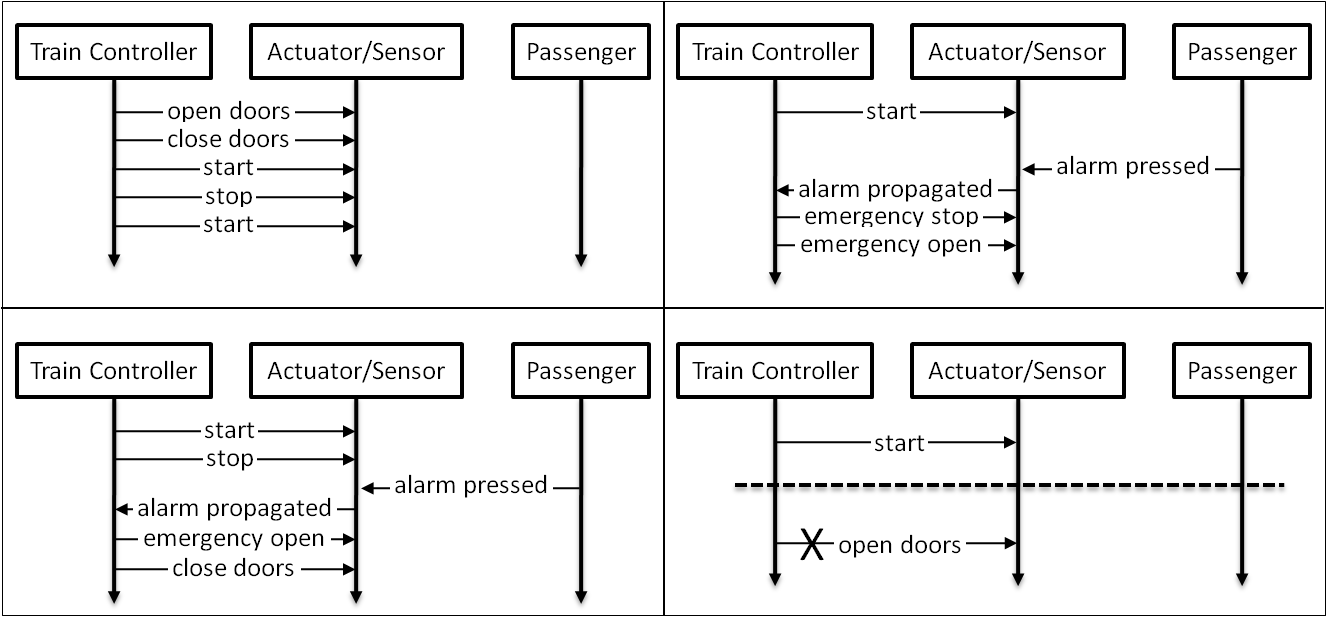
\includegraphics[trim=3mm 3mm 3mm 3mm, clip]{src/4-inductive/images/four-initial-scenarios}}
\caption{Initial positive and negative scenarios for a train system\label{Fig:init:scen}.}
\end{figure}


\item[ChooseStatePair] The candidate solution is refined by merging well- selected state pairs. The \texttt{ChooseStatePair} function determines which pairs to consider. It relies on the standard order $<$ on strings. Each state of the PTA can be labeled by its unique prefix from the initial state. Since prefixes can be sorted according to that order, the states can be ranked accordingly. For example, the PTA states in Fig.~\ref{Fig:algo:steps} are labeled by their rank according to this order. The algorithm considers states $q$ of the PTA in increasing order. The state pairs considered for merging only involve such state $q$ and any state $q'$ of lower rank. The $q'$ states are considered in increasing order as well. This particular ordering is specific to the original RPNI algorithm.

\item[Merge] The \texttt{Merge} function merges the two states $(q, q')$ selected in order to compute a quotient automaton, that is, to generalize the current set of positive behaviors. In the example of Fig.~\ref{Fig:algo:steps}, we assume that states 0, 1, and 2 were previously determined not to be compatible for merging (through negative scenarios initially submitted or generated scenarios that were rejected by the user). Merging a candidate state pair may produce a non-deterministic LTS. For example, after having merged $q = 3$ and $q' = 0$ in the upper part of Fig.~\ref{Fig:algo:steps}, two transitions labeled \texttt{start} from state 0 lead to states 2 and 6, respectively. In such a case, the \texttt{Merge} function merges states 2 and 6 and, recursively, any further pair of states that introduces non-determinism. 

We call \textsl{merging for determinization} this recursive operation of removing non-determinism. This operation guarantees that the current solution at any step is deterministic. It produces an automaton which may accept a more general language than the one it starts from. Therefore, it is not equivalent to the standard algorithm to transform a non deterministic automaton into a deterministic one accepting the same language~\cite{Hopcroft:1979}. Notably, the time complexity of merging for determinization is a linear function of the number of states of the automaton it starts from whereas the standard determinization algorithm is exponential in the worst case. Also, the resulting automaton is still part of the same inductive search space (see Section~\ref{subsection:gi-background-search-space}). 

\begin{figure}
\centering
\scalebox{.67}{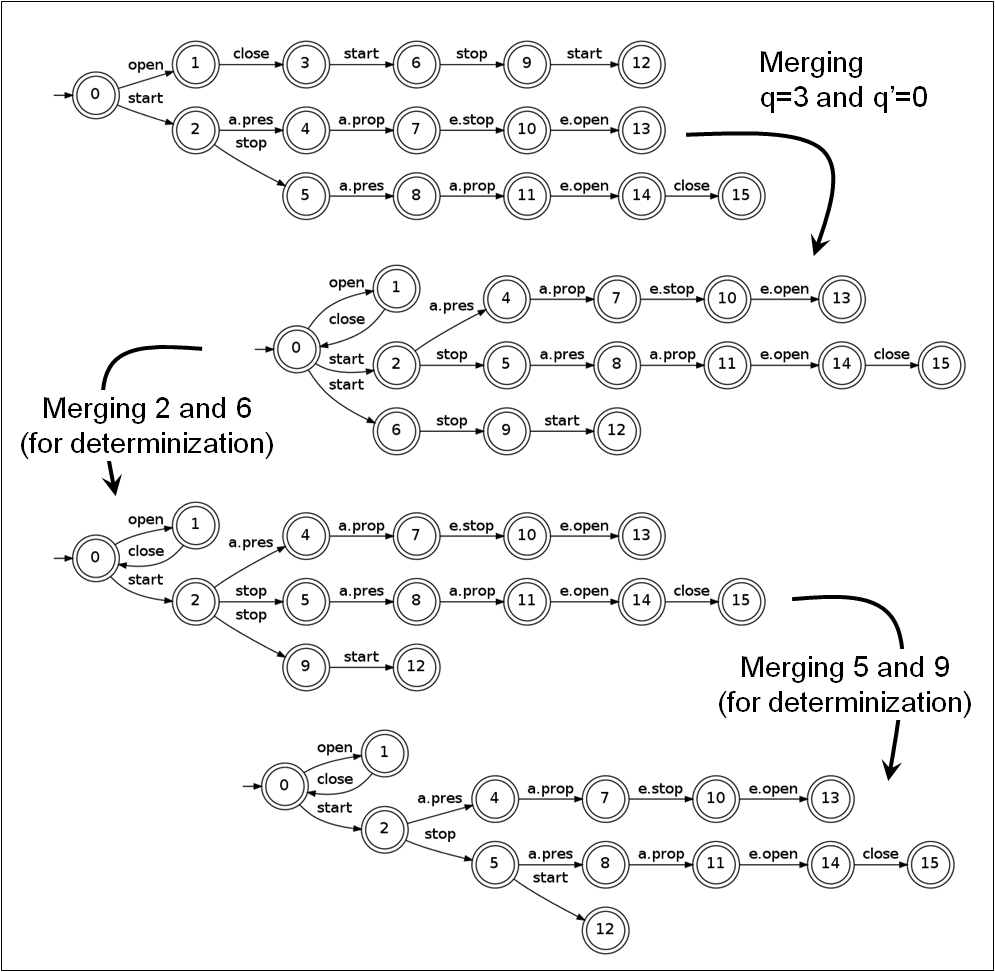
\includegraphics[trim=3mm 3mm 3mm 3mm, clip]{src/4-inductive/images/algo-steps}}
\caption{A typical induction step of the \textsc{QSM} algorithm\label{Fig:algo:steps}.}
\end{figure}

When two states are merged, the rank of the resulting state is defined as the lowest rank of the pair; in particular, the rank of the merged state when merging $q$ and $q'$ is defined as the rank of $q'$ by construction. If no compatible merging can be found between $q$ and any of its predecessor states according to $<$, state $q$ is said to be \textsl{consolidated}. In the example, states 0, 1, and 2 are consolidated.

\item[Consistent] The \texttt{Consistent} function checks whether the automaton $A_{new}$ correctly rejects all negative scenarios. As seen in the pseudo code, the quotient automaton is discarded by \textsc{QSM} when it is detected not to be consistent.

\end{description}

\subsection{Generating queries submitted to the end-user\label{QSM:query}}

This section describes how queries are generated in the \textsc{QSM} algorithm and how the answers provided by the end-user are processed.

\begin{description}

\item[GenerateQuery] When an intermediate solution is consistent with the available scenarios, new scenarios are generated for classification by the end-user as positive or negative. The aim is to avoid poor generalizations by enriching the possibly limited collection of initial scenarios. The notion of characteristic sample drives the identification of which new scenarios should be generated as queries. 

Recall from section~\ref{subsection:gi-background-rpni} that a sample is characteristic of a regular language $L$ if it contains enough positive and negative information. On the one hand, the required positive information is the set of short prefixes $Sp(L)$ which form the shortest histories leading to each state of the canonical automaton $A(L)$. This positive information must also include all elements of the kernel $N(L)$ which represents all system transitions, that is, all shortest histories followed by any admissible event. If such positive information is available, $A(L)$ can always be derived from the PTA by an appropriate set of merging operations. On the other hand, the negative traces provide the necessary information to make incompatible the merging of states which should be kept distinct. A negative trace which would exclude the merging of a state pair $(q, q')$ can be simply made of the shortest history leading to $q'$ followed by any continuation from state $q$ as detailed below.

Consider the current solution of our induction algorithm when a pair of states $(q, q')$ is selected for merging (line 5 in the pseudo code). By construction, $q'$ is always a consolidated state at this step of the algorithm; that is, $q'$ is considered to be in $Sp(L)$. State $q$ is always both the root of a tree and the child of a consolidated state. In other words, $q$ is situated at one letter of a consolidated state, that is, $q$ is considered to be in $N(L)$. States $q$ and $q'$ are compatible according to the available negative scenarios; they would be merged by the standard RPNI algorithm. The QSM extension will first confirm or infirm the compatibility of $q$ and $q'$ by generating scenarios to be classified by the end-user. The generated scenarios are constructed as follows.

\begin{figure}
\centering
\scalebox{.75}{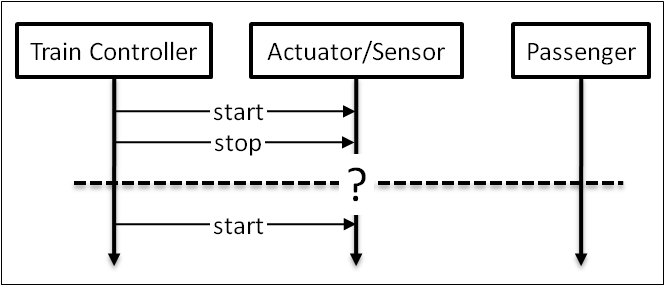
\includegraphics[trim=3mm 3mm 3mm 3mm, clip]{src/4-inductive/images/scenario-question}}
\caption{A new scenario to be classified by the end-user\label{Fig:generated:question}.}
\end{figure}

Let $A$ denote the current solution, $L(A)$ the language generated by $A$, and $A_{new}$ the quotient automaton computed by the \texttt{Merge} function at some given step. Let $x \in Sp(L)$ and $y \in N(L)$ denote the short prefixes of $q'$ and $q$ in A, respectively. Let $u \in L(A)/y$ denote a suffix of $q$ in $A$. 

A generated scenario is built from a system trace $xu$ such that $xu \in L(A_{new})\setminus L(A)$; it can be further decomposed as $xvw$ such that $xv \in L(A)$. The trace $xu$ is thus constructed as the short prefix of $q'$ concatenated with a suffix of $q$ in the current solution, provided the entire behavior is not yet accepted by $A$. Such system trace can be converted to MSC using the structural information provided by a context diagram \cite{Jackson:1995}. The scenario is made of two parts: the first part $xv$ is an already accepted behavior whereas the second part $w$ provides a continuation to be checked for acceptance by the end-user. When submitted to the end-user, the generated scenario can always be rephrased as a question: after having executed the first episode ($xv$), can the system continue with the second episode ($w$)? 

Consider the example in Fig.~\ref{Fig:algo:steps} with selected state pair $q=3, q'=0$. As $q'$ is the root of the PTA, its short prefix is the empty trace $\lambda$. The suffixes of $q$ here yield one generated question (Fig.~\ref{Fig:generated:question}), which can be rephrased as follows: when having started and stopped the train, can the controller restart it? One can see that the first episode of this scenario in Fig.~\ref{Fig:algo:steps} is already accepted by $A$ whereas the entire behavior is accepted in $A_{new}$.

\item[CheckWithEndUser] When a new scenario is generated, it is submitted as a query to the end-user. If the end-user classifies the $Query$ as positive, it is added to the collection of positive scenarios. This addition changes the search space as it extends $S^+$ and consequently the PTA. However, this extension is implicit as the new solution $A_{new}$ is, by construction, also a quotient automaton of this extended PTA. When the $Query$ is classified as negative the induction process is recursively started on the extended scenario collection.

\end{description}

The QSM algorithm has a polynomial time complexity in the size of the learning sample $\mathcal{L}^+(Sc)$, see \cite{Dupont:2008}. 

Moreover, when it receives a characteristic sample in the initial scenario collection it is guaranteed that no additional scenario can be classified as negative. It follows that QSM will not be called recursively anymore and stops by returning the target model. 

An experimental study of the actual sample size required to observe the convergence of \textsc{QSM} and the number of queries submitted to the end-user is detailed in Chapter~\ref{chapter:evaluation}.

\subsection{Reducing the number of queries; the blue-fringe optimization\label{BlueFringe}}

The order in which states are considered for merging by the \texttt{ChooseStatePair} function described in section~\ref{QSM:merging} follows from the implicit assumption that the current sample is characteristic. Consequently, two states are considered compatible for merging if there is no suffix to distinguish among them. This can lead to a significant number of scenarios being generated to the end-user when the initial sample is sparse and actually not characteristic for the target System LTS. 

To overcome this problem, one can use an optimized strategy known as Blue-Fringe~\cite{Lang:1998}. The difference lies in the way state pairs are considered for merging. The general idea is to early detect incompatible state pairs and, subsequently, first consider state pairs for which compatibility has the highest chance to be confirmed by the user through positive classification. The resulting ``please confirm'' interaction may also appear more appealing to the user.

\begin{figure}
\centering
\scalebox{.55}{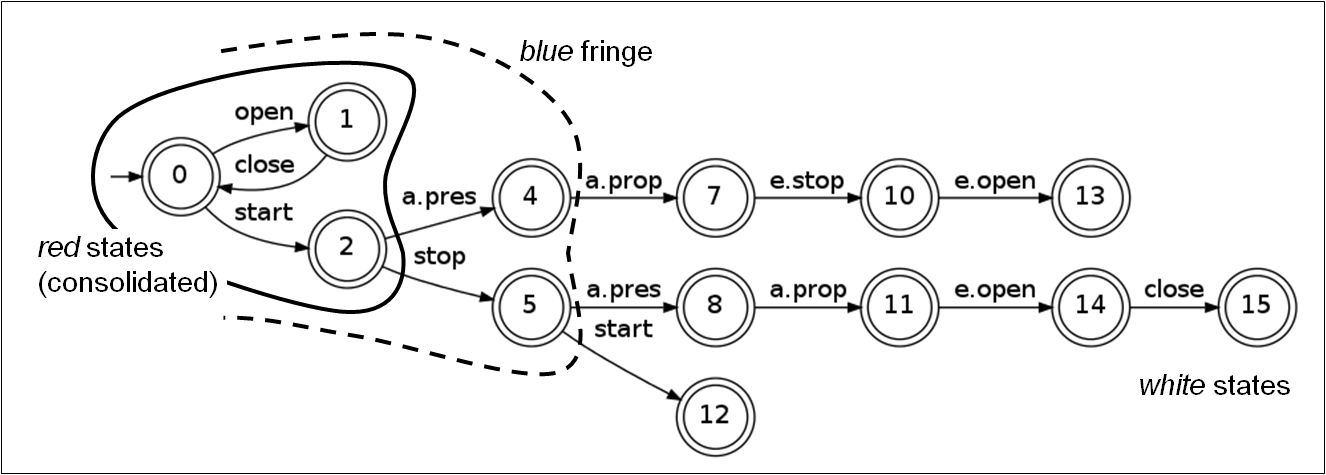
\includegraphics[trim=3mm 3mm 3mm 3mm, clip]{src/4-inductive/images/blue-fringe}}
\caption{Consolidated states (red) and states on the fringe (blue) in a temporary solution\label{Fig:BlueFringe}.}
\end{figure}

Fig.~\ref{Fig:BlueFringe} gives a typical example of a temporary solution produced by the original algorithm. Three state classes can be distinguished in this LTS. The red states are the consolidated ones (0, 1 and 2 in this example). Outgoing transitions from red states lead to blue states unless the latter have already been labeled as red. Blue states form the blue fringe (4 and 5 in this case). All other states are white states. 

The original \texttt{ChooseStatePair} function described in section~\ref{QSM:merging} considers the lowest-rank blue state first (state 4 here) for merge with the lowest-rank red state (0). When this choice leads to a compatible quotient automaton, generated scenarios are submitted to the end-user; in this case, a scenario equivalent to the trace \artifact{<alarm propagated, emergency stop, emergency open>}. The above strategy may lead to multiple queries being generated to avoid poor generalization. Moreover, such queries may be non-intuitive for the user, \textit{e.g.} the \artifact{alarm propagated} event is sent to the train controller without having been fired by the \artifact{alarm pressed} event to the sensor.

To select a state pair for merging, the Blue-Fringe strategy evaluates all (red, blue) state pairs first. The \texttt{ChooseStatePair} function now calls the \texttt{Merge} and \texttt{Compatible} functions before selecting the next state pair. If a blue state is found to be incompatible with all current red states, it is immediately promoted to red; the blue fringe is updated accordingly and the process of evaluating all (red, blue) pairs is iterated. When no blue state is found to be incompatible with red states, the most compatible (red, blue) pair is selected for merging. This is dictated by a scoring mechanism implemented in the \texttt{Compatible} function (see below).

For implementing the Blue-Fringe strategy, it is convenient to adapt \texttt{Initialize} so as to build an \emph{augmented} prefix tree acceptor. Such PTA captures the negative traces in $\mathcal{L}^-(Sc)$ in addition to the positive traces in $\mathcal{L}^+(Sc)$. States reached by a negative trace are tagged as error states; they are depicted in black, as in Fig. \ref{figure:augmented-pta}. 

The \texttt{Compatible} function is also updated to return a compatibility score instead of a boolean value. The score is defined as $-\infty$ when merging the current (red, blue) pair leads to merge an accepting state and an error state during merging for determinization\footnote{in the case of a prefix-closed language, non-error states are all accepting. Recall that this is not necessarily true for any regular language.}; this score indicates an incompatible merging. Otherwise, the compatibility score measures how many accepting states have been merged together. The (red, blue) pair with the highest compatibility score is considered first. The strategy can be further refined with a compatibility threshold $\alpha$ as additional input parameter. Two states are considered to be compatible if their compatibility score is above that threshold. This additional parameter controls the level of generalization since increasing $\alpha$ decreases the number of state pairs that are considered compatible for merging; it thus decreases the number of generated queries.

\begin{figure}\centering
\scalebox{.35}{\includegraphics*{src/4-inductive/images/augmented-pta}}
\caption{Augmented PTA for scenarios in Fig.~\ref{Fig:init:scen}\label{figure:augmented-pta}.}
\end{figure}

Experimental results about the effectiveness of using QSM with and without the Blue-Fringe strategy are detailed in Chapter~\ref{chapter:evaluation}.

\section{Induction of LTS models from hMSCs\label{section:inductive-from-hMSC}}

\section{Discussion\label{section:inductive-discussion}}


